\documentclass[root.tex]{subfiles}

\begin{document}

{\pagestyle{empty}}
\section{\gls{HIL} verification setup}
\label{chap:HiL-Architecture}


In accordance with the process of the V-model \cite{automotive_software_engineering} it was deemed necessary and safest to verify both hardware, software, and the integrated algorithm in cooperation with the system in a \gls{HIL}-test. 

The \gls{VTM} library includes a lot of processing-intensive sub-models (tire models, vehicle parameter sets) which lead to processing power not sufficing to allow for \gls{VTM}'s execution in the dSPACE environment on the \gls{MABII}. To perform \gls{HIL}-testing it was thus necessary to split the computational load and accomplish real-time data exchange between the hardware controlling-system on the \gls{MABII} and the rest of the simulation which will be run parallely in Simulink in real-time on a standard PC. Though there are dedicated real-time platforms available to achieve real-time execution it was decided to rely on a standard PC to minimize costs.% and have a lean work-process without extra steps of code conversion to different platforms.

\begin{figure*}[htb]
	\centering
	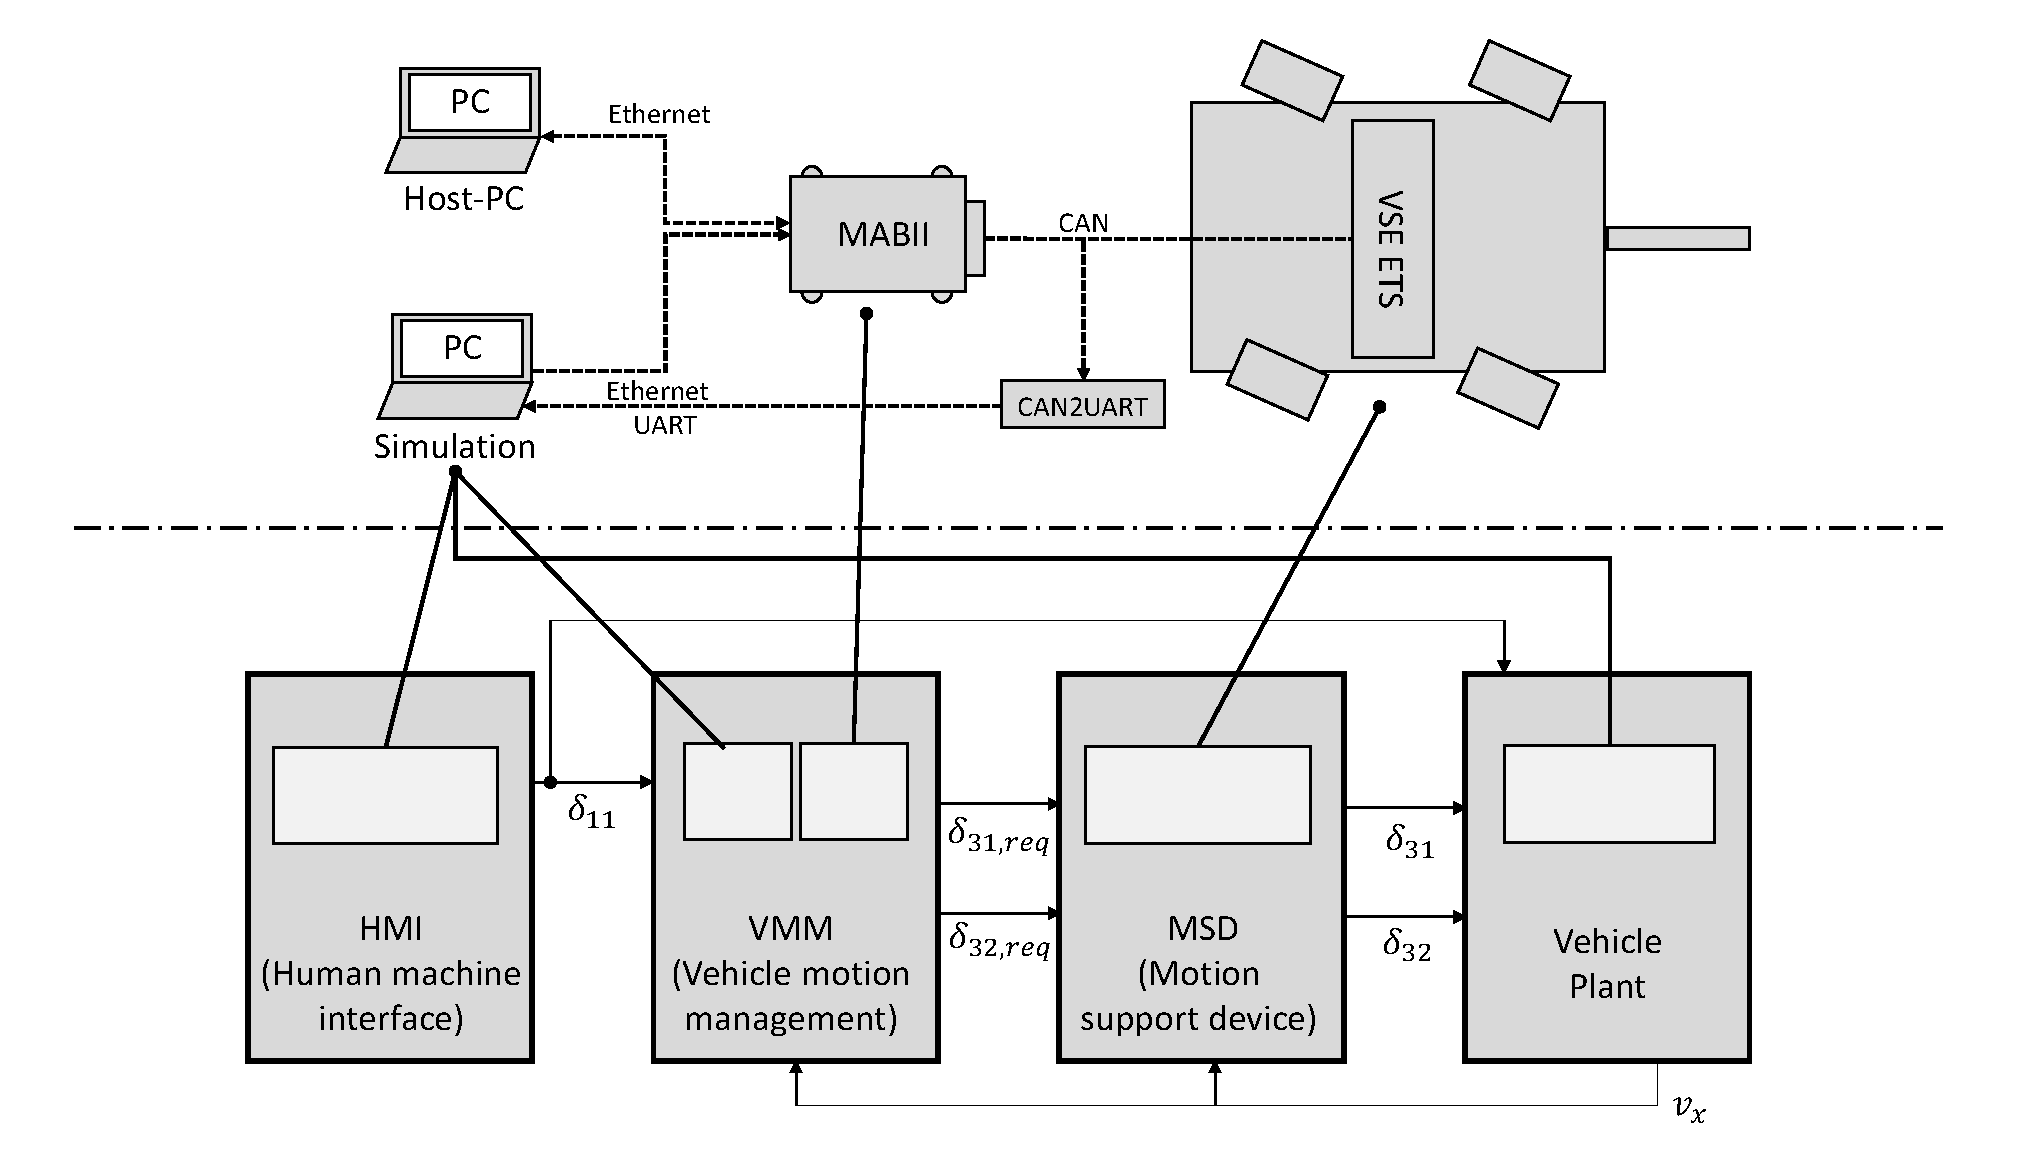
\includegraphics[width=1\linewidth]{HIL_overview}
	\caption[Overview of \acrlong{HIL}-simulation, distribution of sub-functions over different physical platforms (top) and correlation to Volvo functionality architecture (bottom)]{Overview of \gls{HIL}-simulation, distribution of sub-functions over different physical platforms (top) and correlation to Volvo functionality architecture (bottom)}
	
	\label{fig:HIL_overview}
\end{figure*}



 Figure \ref{fig:HIL_overview} illustrates the distribution of the \gls{HIL}-setup's different components according to the Volvo Group Technology functionality model \cite{nilsson2015traffic} over two computers, the \gls{MABII} and the actual hardware (axles, hydraulic control system). The \gls{VMM} consists of the previously developed controller which is executed on the simulation PC and the steering interface executed on the \gls{MABII}. For track-testing it is necessary to also port the controller for execution on the \gls{MABII} to have one closed off system. %This was not yet possible to achieve for the tests at hand, as some components used within the controller algorithm's  Simulink structure were incompatible for real-time execution on the dSPACE system.




\subsection{Modification to base system}
The sensors described in \ref{sec:basevehicle} were discarded and replaced by an artificial signal emulating the original message structure. By using the inverse  function of the original mapping of articulation angle to steering angle, it was possible to command the desired steering angle. The base system has one \gls{CAN} for both axles, resulting in one common steering angle for the both of them. By splitting this \gls{CAN} into two separate networks, it is possible to actuate the axles independently. 


\end{document}